\documentclass[sigconf,10pt,anonymous]{acmart}

\usepackage{microtype}
\usepackage{booktabs,multirow,tabularx,array}
\usepackage{algorithm}
\usepackage{algpseudocode}
\usepackage{graphicx}
\usepackage{subcaption}
\usepackage{xcolor}
\usepackage{tikz}
\usepackage{pgfplots}
\usepackage{enumitem}
\usepackage{url}
\usepackage[nameinlink,capitalize,noabbrev]{cleveref}

\usetikzlibrary{arrows.meta,positioning,calc,fit,backgrounds,shapes.geometric,shapes.symbols,decorations.pathreplacing,patterns,matrix,shadows.blur}
\pgfplotsset{compat=1.18}
\definecolor{pgblue}{HTML}{2F6F9F}
\definecolor{pgbluelight}{HTML}{DCECF6}
\definecolor{pgorange}{HTML}{C95F20}
\definecolor{pgorangelight}{HTML}{F8E2D2}
\definecolor{pggreen}{HTML}{37845A}
\definecolor{pggreenlight}{HTML}{DCEFE3}
\definecolor{pgpurple}{HTML}{76549A}
\definecolor{pgpurplelight}{HTML}{E9E0F2}
\definecolor{pggray}{HTML}{5E6872}
\definecolor{pggraylight}{HTML}{ECEFF1}

\tikzset{
  pgbox/.style={draw=pggray, rounded corners=2pt, line width=.6pt, align=center, font=\footnotesize, minimum height=8mm, inner sep=4pt},
  honest/.style={pgbox, fill=pgbluelight, draw=pgblue},
  attack/.style={pgbox, fill=pgorangelight, draw=pgorange, pattern=north east lines, pattern color=pgorange!28},
  defense/.style={pgbox, fill=pggreenlight, draw=pggreen, double},
  theory/.style={pgbox, fill=pgpurplelight, draw=pgpurple},
  infra/.style={pgbox, fill=pggraylight, draw=pggray},
  dataflow/.style={-{Stealth[length=2.2mm]}, draw=pgblue, line width=.8pt, shorten >=2pt, shorten <=2pt},
  attackflow/.style={-{Stealth[length=2.2mm]}, draw=pgorange, dashed, line width=.8pt, shorten >=2pt, shorten <=2pt},
  controlflow/.style={-{Stealth[length=2.2mm]}, draw=pggreen, double, line width=.55pt, shorten >=2pt, shorten <=2pt},
  theoryflow/.style={-{Stealth[length=2.2mm]}, draw=pgpurple, line width=.7pt, shorten >=2pt, shorten <=2pt},
  flowlabel/.style={font=\scriptsize, fill=white, inner sep=1.5pt, text=black},
  stage/.style={circle, fill=pgpurple, text=white, font=\bfseries\scriptsize, inner sep=1.5pt},
  group/.style={draw=pggray!65, rounded corners=4pt, dashed, inner sep=5pt}
}


% ACM Conference Metadata
\settopmatter{printfolios=true,printacmref=false}
\renewcommand\footnotetextcopyrightpermission[1]{}
\pagestyle{plain}

% Theorem environments (Assumption and Remark are not predefined in acmart)
\newtheorem{assumption}{Assumption}
\theoremstyle{remark}
\newtheorem{remark}{Remark}

% Macros
\newcommand{\PG}{\textsc{PoisonGuard}}
\newcommand{\Prov}{\mathsf{Prov}}
\newcommand{\Allow}{\mathsf{allow}}
\newcommand{\Quarantine}{\mathsf{quarantine}}
\newcommand{\Deny}{\mathsf{deny}}
\newcommand{\Clean}{\mathcal{C}}
\newcommand{\Bad}{\mathcal{B}}
\newcommand{\Events}{\mathcal{E}}
\newcommand{\Graph}{\mathcal{G}}
\newcommand{\Loss}{\mathcal{L}}
\newcommand{\Risk}{\mathcal{R}}
\newcommand{\ind}{\mathbb{I}}

\begin{document}

\title[PoisonGuard: Provenance Selection and Lineage Rollback for On-Device SLMs]{PoisonGuard: Provenance-Carried Data Selection and Lineage Rollback for Poison-Resilient On-Device SLM Personalization}

\author{Anonymous Author(s)}
\affiliation{
  \institution{Institution Withheld for Double-Blind Review}
  \country{}
}

\begin{abstract}
On-device personalization of small language models (SLMs) increasingly combines persistent agent memory with locally fine-tuned LoRA adapters. However, mobile data arrive across channels with disparate trust (typed text, messages, notifications, shared files). Conventional pipelines discard provenance metadata, enabling \emph{cross-sink laundering} where untrusted external payloads enter memory, get selected into training windows, and permanently corrupt model parameters even after raw records are deleted. We present \PG{}, an OS-verifiable, provenance-aware personalization system for mobile SLMs. \PG{} binds immutable provenance envelopes to ingress events, enforces independent sink policies across memory and training, isolates unpromoted adapters in quarantine, and tracks causal dependencies within a unified lineage graph. Upon detecting or revoking poisoned data, \PG{} invalidates contaminated descendants, restores the latest clean checkpoint, and deterministically replays unaffected clean events. We prove that \PG{} guarantees non-laundering under complete mediation and achieves exact counterfactual parameter restoration. Evaluated across five independent seeds on StrategyQA and MemoryGraft, paired with physical Xiaomi 13T hardware measurements, \PG{} neutralizes backdoors ($\mathrm{ASR}=0.0\%$), maintains $70.0\%$ clean utility ($0.0\%$ false quarantine), executes exact rollback in $2.94\text{ ms}$ with only $128\text{ kB}$ storage overhead, and matches $100\%$ of clean parameters, establishing a sound foundation for poison-resilient on-device personalization.

\end{abstract}

\begin{CCSXML}
<ccs2012>
   <concept>
       <concept_id>10002978.10003006.10003007</concept_id>
       <concept_desc>Security and privacy~Mobile and wireless security</concept_desc>
       <concept_significance>500</concept_significance>
   </concept>
   <concept>
       <concept_id>10010147.10010257.10010293</concept_id>
       <concept_desc>Computing methodologies~Machine learning</concept_desc>
       <concept_significance>500</concept_significance>
   </concept>
   <concept>
       <concept_id>10011007.10010940.10010992</concept_id>
       <concept_desc>Software and its engineering~Software organization and properties</concept_desc>
       <concept_significance>300</concept_significance>
   </concept>
 </ccs2012>
\end{CCSXML}

\ccsdesc[500]{Security and privacy~Mobile and wireless security}
\ccsdesc[500]{Computing methodologies~Machine learning}
\ccsdesc[300]{Software and its engineering~Software organization and properties}

\keywords{On-device SLM personalization, data poisoning, provenance, agent memory, LoRA adapters, adapter quarantine, lineage rollback}

\maketitle
\thispagestyle{plain}
\pagestyle{plain}

% Core paper sections (Main content: target <= 12 pages)
\section{Introduction}
\label{sec:introduction}

Personalization is moving from a transient prompt into persistent model state. A mobile assistant may retrieve an old message, cache a preference as memory, or update a compact adapter with examples selected from recent interactions. Parameter-efficient adaptation makes the last option technically plausible: LoRA confines updates to low-rank matrices \cite{hu2021lora}, QLoRA lowers memory demand further \cite{dettmers2023qlora}, and prototype systems now demonstrate local fine-tuning on phones \cite{peng2024pocketllm,geng2025mobilefinetuner}. Personalization benchmarks such as LaMP formalize the utility side of this trend \cite{salemi2023lamp}. These capabilities are useful precisely because a phone sees data that a server does not.

The same locality creates an unusually sharp integrity problem. A phone sees user-authored text, but it also sees remote content delivered as messages, notifications, invitations, shared files, clipboard transfers, and OCR-indexed screenshots. The operating system can often distinguish those origins at ingestion time. Once content is converted to a plain training example or summarized into a memory record, however, the distinction can disappear. A received message can consequently influence a reply model as if it were a user preference. If that memory later becomes an adapter-training example, deleting the message or memory no longer removes the learned behavior.

This paper calls that transition \emph{cross-sink laundering}. The term is narrower than generic data poisoning. It denotes a causal path from an untrusted source, through one persistent learning sink, into another sink whose state survives cleanup of the first. AgentPoison shows that poisoned memories or knowledge bases can steer retrieval-augmented agents \cite{chen2024agentpoison}; MINJA demonstrates query-only memory injection \cite{dong2025minja}; recent work studies stealthy email injection, self-reinforcing memories, and poisoned experience retrieval \cite{zhang2026memghost,yang2026zombie,srivastava2025memorygraft}. SkillJack is particularly close conceptually: an agent can transform poisoned trajectories into reusable skills that outlive source deletion \cite{ying2026skilljack}. PoisonGuard asks the mobile-learning analogue: what happens when a memory record becomes a gradient update to a locally trained LoRA adapter?

Existing defenses do not directly enforce this boundary. Memory-only filters can reject or down-rank suspicious records \cite{sunil2026memorypoison,wei2025amemguard}, and isolation can stop external data from entering a privileged agent context \cite{wen2026agentsys}. Textual backdoor detectors inspect inputs or behavior \cite{qi2020onion,yang2021rap}, while spectral or activation statistics inspect learned representations \cite{tran2018spectral,chen2018activation}. Federated robust aggregation compares updates from multiple clients \cite{blanchard2017krum,yin2018byzantine,pillutla2019rfa,cao2020fltrust}, but a single phone has no worker population or trusted server reference. Approximate unlearning is also an unsafe synonym for restoration: empirical evidence shows that practical unlearning methods may leave poisoning effects behind \cite{pawelczyk2025unlearning}. These methods remain valuable baselines, but none answers which downstream state consumed a later-revoked local item.

\PG treats provenance as a control-plane object rather than a descriptive log. Every ingested event carries an envelope containing channel class, application identity, remote principal when available, user-authorship evidence, capture time, integrity metadata, and derivation parents. A policy returns one of three decisions for each sink: admit, quarantine, or deny. Memory and adapter training consult the same provenance graph. Candidate adapters are never promoted directly; they are trained against a versioned window, subjected to behavioral and update-level audits, and promoted only when the policy and audit gate both pass. Each promoted checkpoint records the exact source-event closure that influenced it.

Revocation therefore becomes graph invalidation followed by rollback-and-replay. When an item is found malicious, PoisonGuard identifies all descendants, chooses the newest checkpoint outside the invalidated closure, restores it, and replays later admissible events with pinned code, model, optimizer, tokenizer, and randomness. This is more expensive than deleting a row but makes the recovery claim testable. We state the conditions under which the recovered memory and adapter equal the counterfactual state that would have arisen had the poison never been admitted. We also identify the conditions under which this statement fails.

\paragraph{Contributions.} This manuscript develops five contributions locked to the original PoisonGuard concept.

\begin{enumerate}
  \item We formalize a single-device, multi-channel threat model for mixed memory-plus-adapter personalization and define cross-sink laundering, including persistence after source deletion.
  \item We design a provenance-carried selection plane that preserves source and derivation information from mobile ingestion through memory construction, training-window selection, candidate adapters, and promoted checkpoints.
  \item We introduce quarantine-then-promote adapter training and a shared lineage store that supports causal invalidation across both persistent sinks.
  \item We give sufficient-condition theorems for non-laundering and exact rollback-and-replay, together with explicit bounds on contaminated influence, checkpoint storage, and replay work. The claims are conditional, not optimality results.
  \item We specify an implementable evaluation on Android-class phones, including channel-adapted memory and LoRA poisoning, an adaptive user-retyping attacker, and systems metrics. No fabricated device results are reported.
\end{enumerate}

\paragraph{Scope and non-goals.} PoisonGuard does not protect a compromised OS or training runtime. It does not prove that content is semantically truthful. It does not solve generic prompt injection, privacy leakage, or federated Byzantine aggregation. It cannot distinguish a genuine user choice from a user action induced by social engineering without additional confirmation. Its strongest result is counterfactual restoration under explicit reproducibility assumptions, not universal prevention.

\paragraph{Road map.} \Cref{sec:related} positions the work. \Cref{sec:preliminaries,sec:system} define notation and the system. \Cref{sec:problem} formalizes laundering and objectives. \Cref{sec:method} presents the design, \cref{sec:theory} analyzes it, and \cref{sec:algorithms} gives executable procedures. \Cref{sec:experiments} specifies the evaluation; \cref{sec:discussion,sec:limitations} discuss deployment and limitations.

\begin{figure*}[t]
  \centering
  \resizebox{0.95\textwidth}{!}{\resizebox{\linewidth}{!}{%
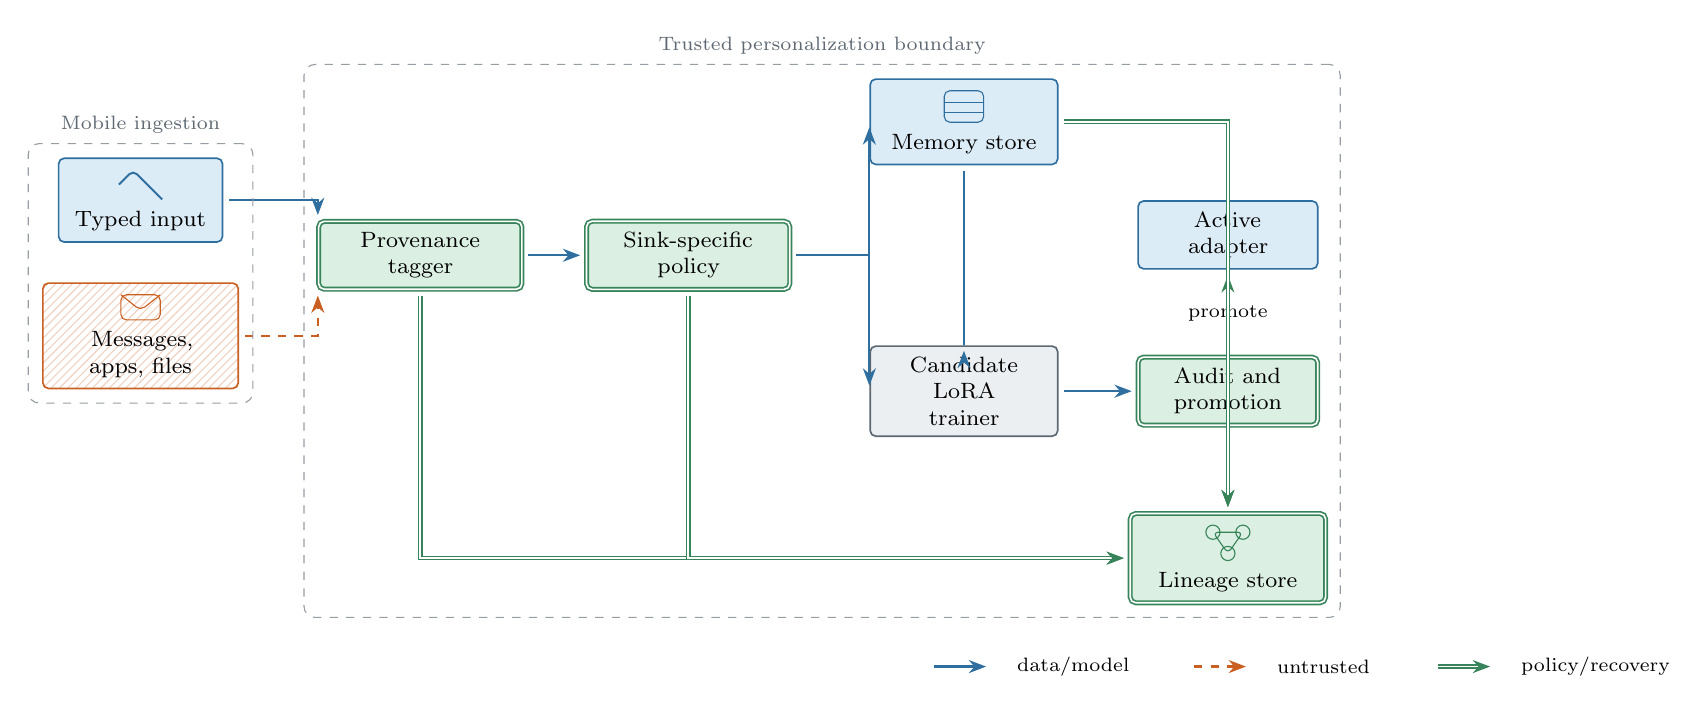
\begin{tikzpicture}[node distance=7mm and 8mm, every node/.style={transform shape}]
  \node[honest, text width=18mm] (typed) {\tikz\draw[pgblue,line width=.7pt] (0,0)--(.18,.18)--(.55,-.19);\\Typed input};
  \node[attack, text width=22mm, below=5mm of typed] (remote) {\tikz{\draw[pgorange] (0,0) rectangle (.5,.32); \draw[pgorange] (0,.32)--(.25,.12)--(.5,.32);}\\Messages, apps, files};
  \node[defense, text width=23mm, right=12mm of typed, yshift=-7mm] (tag) {Provenance\\tagger};
  \node[defense, text width=23mm, right=of tag] (policy) {Sink-specific\\policy};
  \node[honest, text width=21mm, above right=7mm and 10mm of policy] (memory) {\tikz{\draw[pgblue] (-.25,-.2) rectangle (.25,.2); \draw[pgblue] (-.25,.05)--(.25,.05) (-.25,-.08)--(.25,-.08);}\\Memory store};
  \node[infra, text width=21mm, below right=7mm and 10mm of policy] (trainer) {Candidate LoRA\\trainer};
  \node[defense, text width=20mm, right=10mm of trainer] (audit) {Audit and\\promotion};
  \node[honest, text width=20mm, above=11mm of audit] (active) {Active\\adapter};
  \node[defense, text width=22mm, below=11mm of audit] (lineage) {\tikz\draw[pggreen] (0,0) circle (.09) (.38,0) circle (.09) (.19,-.27) circle (.09) (0,0)--(.38,0)--(.19,-.27)--cycle;\\Lineage store};

  \draw[dataflow] (typed.east) -| (tag.north west);
  \draw[attackflow] (remote.east) -| (tag.south west);
  \draw[dataflow] (tag.east) -- (policy.west);
  \draw[dataflow] (policy.east) -| (memory.west);
  \draw[dataflow] (policy.east) -| (trainer.west);
  \draw[dataflow] (memory.south) |- (trainer.north);
  \draw[dataflow] (trainer.east) -- (audit.west);
  \draw[controlflow] (audit.north) -- node[flowlabel]{promote} (active.south);
  \draw[controlflow] (tag.south) |- (lineage.west);
  \draw[controlflow] (policy.south) |- (lineage.west);
  \draw[controlflow] (memory.east) -| (lineage.north);
  \draw[controlflow] (audit.south) -- (lineage.north);

  \node[group, fit=(typed)(remote), label={[font=\scriptsize,text=pggray]above:Mobile ingestion}] {};
  \node[group, fit=(tag)(policy)(memory)(trainer)(audit)(active)(lineage), label={[font=\scriptsize,text=pggray]above:Trusted personalization boundary}] {};
  \coordinate (leg) at ($(lineage.south)+(0,-8mm)$);
  \draw[dataflow] ($(leg)+(-38mm,0)$)--($(leg)+(-30mm,0)$);
  \node[font=\scriptsize, anchor=west] at ($(leg)+(-28mm,0)$) {data/model};
  \draw[attackflow] ($(leg)+(-5mm,0)$)--($(leg)+(3mm,0)$);
  \node[font=\scriptsize, anchor=west] at ($(leg)+(5mm,0)$) {untrusted};
  \draw[controlflow] ($(leg)+(26mm,0)$)--($(leg)+(34mm,0)$);
  \node[font=\scriptsize, anchor=west] at ($(leg)+(36mm,0)$) {policy/recovery};
\end{tikzpicture}%
}
}
  \caption{PoisonGuard architecture. Blue solid arrows carry ordinary data, orange dashed arrows show potential adversarial flow, and green double-line arrows denote policy or recovery control. Provenance remains attached across both memory and adapter sinks.}
  \label{fig:architecture}
\end{figure*}

\section{Related Work and Novelty Boundary}
\label{sec:related}

The relevant literature spans persistent agent memory, poisoning and backdoors, parameter-efficient personalization, provenance, unlearning, and federated robustness. The boundary matters: PoisonGuard is neither a new trigger-generation attack nor a federated aggregation rule. It is a lifecycle mechanism for a single device where one source item may influence two persistent sinks.

\subsection{Persistent memory and retrieval poisoning}

Retrieval-augmented generation combines parametric and retrieved knowledge \cite{lewis2020rag}. Agent systems extend this idea into longer-lived state: Generative Agents store and reflect over experience \cite{park2023generativeagents}, MemoryBank maintains long-term conversational memory \cite{zhong2023memorybank}, MemGPT manages context as an operating-system-like hierarchy \cite{packer2023memgpt}, and Reflexion converts feedback into reusable verbal memory \cite{shinn2023reflexion}. A survey by Zhang et al. organizes the growing design space of agent memory \cite{zhang2024memorysurvey}. These systems motivate persistent personalization but do not make mobile channel origin an enforceable training policy.

PoisonedRAG demonstrates that an attacker can corrupt retrieval by injecting carefully chosen texts \cite{zou2024poisonedrag}. AgentPoison optimizes triggers that retrieve malicious demonstrations from an agent memory or knowledge base \cite{chen2024agentpoison}. MINJA injects malicious records through query-only interaction \cite{dong2025minja}. Later work broadens the persistence surface. MemoryGraft targets stored experiences \cite{srivastava2025memorygraft}; Zombie Agents turns one-time external exposure into self-reinforcing memory \cite{yang2026zombie}; GhostWriter plants and later activates memory payloads in tool-using personal agents \cite{torres2026ghostwriter}; and MemGhost studies stealthy single-email delivery into persistent personal agents \cite{zhang2026memghost}. SPORE addresses extraction rather than integrity, but underscores that memory interfaces create cross-session attack paths \cite{gao2026spore}.

SkillJack supplies the closest empirical analogy to laundering: poisoned trajectories are transformed into reusable skills, become less detectable, and can survive deletion of the original records \cite{ying2026skilljack}. PoisonGuard transfers this question to mobile parameter updates and makes the source-to-weight dependency explicit. It does not claim that SkillJack already evaluated LoRA weights; it did not.

\subsection{Memory and prompt-injection defenses}

Recent defenses filter, isolate, or validate persistent content. A trust-score and temporal-decay defense studies realistic memory-bank contamination \cite{sunil2026memorypoison}. A-MemGuard combines consensus-based validation with a dual-memory design \cite{wei2025amemguard}. AgentSys isolates worker contexts and restricts what returns to a privileged context \cite{wen2026agentsys}. DASGuard traces control-like content in files back to its origin before committing state \cite{tan2026dasguard}. These works support the premise that origin and lifecycle control matter, while leaving open the specific relation between mobile ingestion, training-data selection, and adapter checkpoints.

Prompt-injection defenses address a neighboring boundary. Spotlighting marks untrusted data so a model can distinguish it from instructions \cite{hines2024spotlighting}; StruQ separates instructions and data through structured queries \cite{chen2024struq}; AgentDojo supplies realistic tool-use tasks and attack cases \cite{debenedetti2024agentdojo}. PoisonGuard can host these checks inside its audit gate, but its primary invariant is different: no derived persistent state may lose the provenance of an influencing event.

\subsection{Adapter poisoning and textual backdoors}

Modern candidate SLMs inherit the Transformer architecture \cite{vaswani2017attention}. LoRA makes adaptation compact by representing a weight update as a low-rank product \cite{hu2021lora}; QLoRA couples low-rank adaptation with quantization \cite{dettmers2023qlora}. LoRATK shows that malicious LoRAs can retain backdoors when merged with benign task adapters \cite{liu2024loratk}. Token-level adapter experiments show that poisoned local training data can create backdoors while leaving clean task performance largely unchanged, and that behavioral and weight-level statistics offer complementary signals \cite{lelle2026token}. Gradient Assembly Poisoning targets the factorization itself in distributed LoRA systems \cite{dong2026gap}; its federated attacker differs from PoisonGuard's content-origin attacker, so we use it only to motivate factor-aware auditing.

The broader backdoor literature establishes that small poisoned subsets can implant trigger-conditioned behavior. BadNets identifies supply-chain vulnerability \cite{gu2017badnets}; targeted and clean-label attacks show that labels need not be visibly inconsistent \cite{chen2017targetedbackdoor,shafahi2018poisonfrogs}; and weight poisoning targets pretrained NLP models \cite{kurita2020weightpoison}. NeuBA operates at neuron level in pretrained language models \cite{zhang2021neuba}. Detection methods include spectral signatures \cite{tran2018spectral}, activation clustering \cite{chen2018activation}, influence functions \cite{koh2017influence}, STRIP's input perturbations \cite{gao2019strip}, and textual defenses such as ONION and RAP \cite{qi2020onion,yang2021rap}. PoisonGuard does not assume any one detector is complete. It uses detection to decide promotion and uses lineage for recovery after detection.

\subsection{On-device personalization}

MobileBERT demonstrated that language models can be engineered for resource-constrained inference \cite{sun2020mobilebert}. PocketLLM evaluates derivative-free local fine-tuning on a smartphone \cite{peng2024pocketllm}; MobileFineTuner provides a mobile-native framework for full and parameter-efficient training \cite{geng2025mobilefinetuner}; XPerT reduces local personalization cost through model selection \cite{wang2025xpert}; and recent hypernetwork work synthesizes personalized LoRAs on-device \cite{augenstein2026hyperlora}. LaMP supplies personalization tasks \cite{salemi2023lamp}, while PersonaChat and AESLC provide dialogue and email-like text workloads \cite{zhang2018personachat,zhang2019aeslc}. Qwen2.5 and Gemma 3 define candidate compact model families \cite{qwen2024qwen,gemma2025gemma}. This literature establishes feasibility, not deployed prevalence. Accordingly, our evaluation claims a prototype study rather than universal production coverage.

\subsection{Unlearning, rollback, and provenance}

Machine unlearning seeks to remove the effect of designated examples. SISA partitions training to limit retraining scope \cite{bourtoule2021machineunlearning}; certified removal provides model-specific guarantees \cite{guo2020certified}; adversarial evaluation exposes weaknesses of inexact methods \cite{goel2022adversarialunlearning}; and approximate LLM methods include task-specific forgetting and negative preference optimization \cite{eldan2023harry,zhang2024npo}. Most importantly for this work, Pawelczyk et al. find that practical approximate methods can fail to eliminate poisoning effects \cite{pawelczyk2025unlearning}. PoisonGuard therefore does not call a gradient-based forgetting step ``rollback.'' It restores a pre-influence checkpoint and re-executes a versioned clean suffix.

Data provenance traditionally records where outputs came from and how they were derived. PoisonGuard adopts that causal viewpoint but narrows it to stateful mobile learning. The lineage graph is not a blockchain and does not require distributed consensus. Its purpose is complete mediation, reachability-based invalidation, and deterministic replay.

\subsection{Federated robustness as an inapplicable contrast}

Federated averaging coordinates many clients through a server \cite{mcmahan2017fedavg}. Krum, coordinate-wise robust statistics, Bulyan, and geometric-median aggregation resist some Byzantine update models \cite{blanchard2017krum,yin2018byzantine,mhamdi2018bulyan,pillutla2019rfa}. FLTrust bootstraps trust from a server dataset \cite{cao2020fltrust}; FLAME clusters and clips updates before adding noise \cite{nguyen2021flame}; and FoolsGold addresses sybil-like similarity \cite{fung2018sybil}. Model-poisoning and backdoor studies illustrate the limits of aggregation \cite{bhagoji2018federated,bagdasaryan2020backdoorfl}. More recent federated instruction-tuning work shows that low-concentration poisoned data spread across nominally benign clients can evade defenses designed for malicious clients \cite{zhao2026fedbit}. These methods assume multiple updates to compare. A single phone learning from its own mixed-trust streams has neither that population nor a server root dataset. PoisonGuard cites them to delimit the problem, not as fair head-to-head baselines.

\begin{table}[t]
\centering
\small
\caption{Novelty boundary across related literature.}
\label{tab:boundary}
\resizebox{\columnwidth}{!}{%
\begin{tabular}{lccccc}
\toprule
Family & Memory & Adapter & Provenance & Cross-sink & Exact replay \\
\midrule
Memory/RAG attacks \cite{chen2024agentpoison,dong2025minja,zou2024poisonedrag} & \checkmark & -- & limited & -- & -- \\
Persistent-agent attacks \cite{zhang2026memghost,ying2026skilljack} & \checkmark & skill & motivates & partial & -- \\
Memory defenses \cite{sunil2026memorypoison,wei2025amemguard} & \checkmark & -- & trust signal & -- & -- \\
Adapter defenses \cite{tran2018spectral,lelle2026token} & -- & \checkmark & -- & -- & -- \\
Approximate unlearning \cite{eldan2023harry,zhang2024npo} & -- & \checkmark & deletion set & limited & -- \\
\PG{} (this work) & \checkmark & \checkmark & \checkmark & \checkmark & \checkmark \\
\bottomrule
\end{tabular}%
}
\end{table}

\section{Preliminaries and Notation}
\label{sec:preliminaries}

We consider a single physical device. Time is divided into ingestion events rather than synchronized training rounds. Let $\Events=(e_1,e_2,\ldots)$ be the append-only logical event sequence. An event is not merely text; it includes content, origin, and integrity metadata.

\begin{definition}[Provenance-labelled event]
An event is a tuple
\begin{equation}
e_i=(x_i,\tau_i,a_i,c_i,s_i,u_i,h_i,P_i),
\label{eq:event}
\end{equation}
where $x_i$ is content or a content digest, $\tau_i$ is capture time, $a_i$ is the producing application identity, $c_i$ is a channel class, $s_i$ is a sender or remote principal when available, $u_i\in\{0,1,\bot\}$ records verified user authorship, $h_i$ binds the canonical payload and metadata, and $P_i\subseteq\{e_j:j<i\}$ are derivation parents.
\end{definition}

The channel set is
\begin{equation}
\mathcal{K}=\{\textsf{typed},\textsf{sms},\textsf{notification},\textsf{calendar},\textsf{share},\textsf{clipboard},\textsf{screenshot},\textsf{derived}\}.
\end{equation}
The concrete Android mechanism used to populate each field is an implementation choice; the formal requirement is that the field cannot be rewritten by the untrusted producer after capture.

The system has two persistent learning sinks. A memory state $M_t$ contains records used at inference time. An adapter state $\theta_t=\theta_0+\Delta_t$ augments a frozen base model with a low-rank update. For a weight matrix $W\in\mathbb{R}^{d_o\times d_i}$, LoRA represents
\begin{equation}
W'=W+\alpha B A/r,\qquad A\in\mathbb{R}^{r\times d_i},\quad B\in\mathbb{R}^{d_o\times r}.
\label{eq:lora}
\end{equation}
The dimension statement is important: the lineage mechanism tracks the data that produced the pair $(A,B)$ and the resulting effective update $BA$, not only a serialized adapter filename.

For sink $z\in\{\mathsf{mem},\mathsf{train}\}$, the policy
\begin{equation}
\pi_z(e,\sigma_t)\in\{\Allow,\Quarantine,\Deny\}
\label{eq:policy}
\end{equation}
maps an event and policy state $\sigma_t$ to a decision. Decisions can differ by sink: a received email may be retrievable under an untrusted-data wrapper yet prohibited from training.

\begin{definition}[Lineage graph]
The lineage graph at time $t$ is a directed acyclic graph $\Graph_t=(V_t,E_t)$ whose typed vertices are source events, derived memory records, training examples, windows, audit records, candidate adapters, and promoted checkpoints. An edge $(v,w)$ states that $w$ was computed using $v$ or that $w$'s validity depends on $v$.
\end{definition}

For $S\subseteq V_t$, let $\operatorname{Desc}_{\Graph_t}(S)$ include $S$ and every vertex reachable from it. A revocation set $R_t$ invalidates this descendant closure. The clean event set after revocation is
\begin{equation}
\Clean_t(R_t)=\{e_i:i\le t,\ e_i\notin\operatorname{Desc}_{\Graph_t}(R_t),\ \pi(e_i,\sigma_t)\ne\Deny\}.
\end{equation}

\begin{table}[t]
\centering
\caption{Frequently used notation.}
\label{tab:notation}
\begin{tabularx}{\linewidth}{lX}
\toprule
Symbol & Meaning \\
\midrule
$e_i,x_i,\Prov(e_i)$ & event, payload, and provenance envelope \\
$M_t,\theta_t$ & memory and promoted adapter after logical time $t$ \\
$\pi_z$ & sink-specific admission policy \\
$\Graph_t$ & shared typed lineage graph \\
$W_k$ & $k$th adapter-training window \\
$q_k,\hat\theta_k$ & candidate checkpoint and audited/promotion state \\
$R_t$ & revoked vertices or sources \\
$\operatorname{Desc}(R_t)$ & invalidated lineage closure \\
$\mathcal{A}$ & attack procedure and trigger distribution \\
$\mathrm{ASR}$ & trigger-conditioned attack success rate \\
$U$ & clean personalization utility \\
$C_S,C_T,C_E$ & storage, elapsed-time, and energy costs \\
\bottomrule
\end{tabularx}
\end{table}

\paragraph{Topic-alignment checkpoint.} This section defines every object required by the locked signature: mobile-channel provenance, memory, LoRA state, per-sink selection, shared lineage, and rollback inputs. It introduces no federated or privacy objective.

\section{System and Threat Model}
\label{sec:system}

\subsection{Personalization lifecycle}

The device runs a frozen or infrequently updated base SLM and maintains two mutable forms of personalization. First, a local memory service stores selected records and retrieves them into inference context. Second, a trainer periodically forms a window $W_k$ and produces a candidate LoRA adapter $q_k$. A promotion pointer selects at most one candidate as the active adapter. The two sinks may operate at different cadences, but they share a lineage service and policy state.

\Cref{fig:architecture} separates the data plane from the control plane. Raw content is captured at a trusted ingress boundary. The provenance tagger canonicalizes the payload, retrieves OS-observable attributes, and creates an authenticated envelope. The policy engine issues sink-specific decisions. Derived summaries inherit all parents rather than receiving a fresh ``trusted'' label. The memory service and trainer emit lineage edges transactionally with their state changes. The audit harness evaluates a candidate without exposing it as the active model. Promotion commits the candidate, audit report, and lineage root atomically.

\subsection{Trust assumptions}

\begin{assumption}[Trusted computing base]
\label{ass:tcb}
The mobile OS kernel, provenance service, secure storage used for graph roots, base-model loader, policy engine, lineage recorder, and training runtime execute as specified. Untrusted applications cannot forge another app identity or rewrite a committed event envelope.
\end{assumption}

\begin{assumption}[Complete mediation]
\label{ass:mediation}
Every state-changing operation on memory, training data, candidate adapters, audit decisions, and promoted checkpoints is mediated by the policy/lineage layer. There is no side channel that writes persistent learned state without producing the corresponding lineage edges.
\end{assumption}

\begin{assumption}[Append-only event identity]
\label{ass:identity}
Each event and derived object has a collision-resistant content identifier over its canonical payload, provenance envelope, parent identifiers, and version. Mutation creates a new object rather than changing the old identifier.
\end{assumption}

These assumptions are strong but inspectable. If a vendor allows an application to write directly to the training cache, or if a summarizer discards its parent list, the main guarantee does not apply. PoisonGuard is therefore a system architecture, not a classifier that compensates for arbitrary implementation bypasses.

\subsection{Adversary}

The adversary controls content delivered through one or more non-user channels. It may send messages or calendar invitations, trigger notifications through a malicious app, share files, place text on a synchronized clipboard, or induce content that later appears in a screenshot index. It knows the broad policy and may adapt payloads after observing normal model behavior. It can attempt a memory attack, a training-data backdoor, or a two-stage laundering attack.

The adversary may also socially engineer the user into reproducing a trigger in typed text. This capability is treated separately because the resulting OS evidence legitimately records user authorship. A defense that silently equates ``typed'' with ``benign'' would conceal this residual risk. Our evaluation therefore reports direct-channel and induced-user attacks separately.

The attacker cannot compromise the TCB in \cref{ass:tcb}, forge event authentication, extract secure storage, alter the experiment harness, or physically modify the device. Denial of service through unbounded incoming content is rate-limited but is not the central goal.

\subsection{Assets and security properties}

The principal asset is behavioral integrity of the personalized SLM. Confidentiality and privacy remain important but are not the theorem target. We require four properties.

\begin{definition}[Provenance preservation]
For every persistent object $v$, the graph contains a path from each direct or indirect source event that influenced $v$ to $v$.
\end{definition}

\begin{definition}[Non-laundering]
If policy denies event $e$ for adapter training, then no promoted checkpoint may be a descendant of $e$. If $e$ is later revoked, no checkpoint descendant may remain active after recovery completes.
\end{definition}

\begin{definition}[Quarantine safety]
A candidate adapter cannot serve ordinary user inference before a successful audit and an atomic promotion that records its lineage closure.
\end{definition}

\begin{definition}[Counterfactual restoration]
After revoking $R_t$, the recovered state equals the state obtained by executing the same versioned personalization pipeline on the admissible event subsequence with the revoked lineage closure removed.
\end{definition}

Counterfactual restoration is stronger than ``attack success decreased'' and narrower than semantic repair. Equality may be bitwise for deterministic integer kernels or within a declared tolerance for deterministic floating-point schedules. The experiment must state which form it checks.

\subsection{Deployment boundary}

The design fits a system service, a privileged personalization framework, or a research runtime. A third-party application can implement a weaker variant, but cannot reliably attribute cross-application content without OS support. For that reason, application identity and user-authorship evidence are observations from the trusted ingress boundary rather than strings supplied by the text producer.

\paragraph{Topic-alignment checkpoint.} The architecture remains single-device and mobile. Federated workers, cloud aggregation, and differential privacy are outside the state machine.

\begin{figure}[t]
  \centering
  \resizebox{0.95\columnwidth}{!}{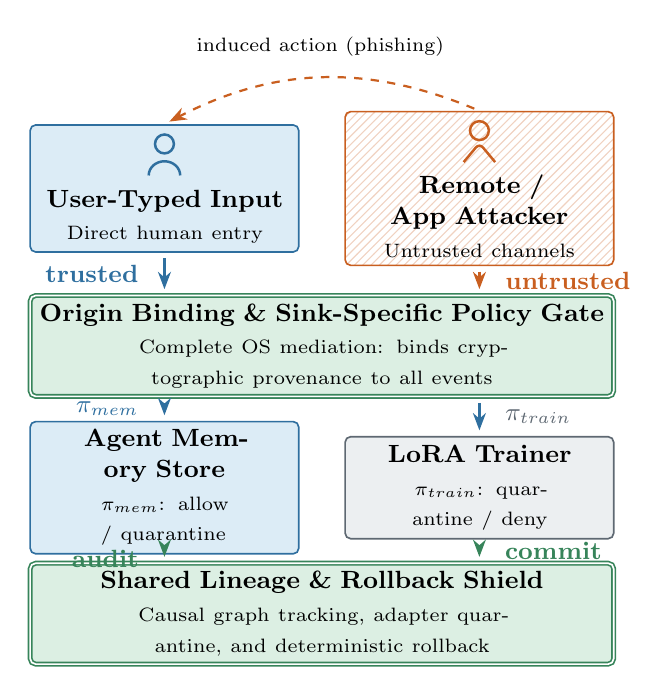
\begin{tikzpicture}[
  hnode/.style={honest, font=\small, text width=32mm, minimum height=9.5mm, inner sep=3pt},
  anode/.style={attack, font=\small, text width=32mm, minimum height=9.5mm, inner sep=3pt},
  dnode/.style={defense, font=\small, text width=72mm, minimum height=9.5mm, inner sep=3pt},
  inode/.style={infra, font=\small, text width=32mm, minimum height=9.5mm, inner sep=3pt}
]
  % Tier 1: Ingress Sources (Side-by-side, y = 0)
  \node[hnode] (user) at (0, 0) {\tikz\draw[pgblue,line width=.9pt] (0,.15) circle (.12) (-.2,-.25) arc (180:0:.2 and .18);\\\textbf{User-Typed Input}\\[0.3mm]\scriptsize Direct human entry};
  \node[anode] (attacker) at (4.0, 0) {\tikz\draw[pgorange,line width=.9pt] (0,.15) circle (.12) (-.2,-.25)--(0,-.01)--(.2,-.25);\\\textbf{Remote / App Attacker}\\[0.3mm]\scriptsize Untrusted channels};

  % Tier 2: Policy & Mediation Gate (y = -2.0) -> Arrow length = 11mm!
  \node[dnode] (guard) at (2.0, -2.0) {\textbf{Origin Binding \& Sink-Specific Policy Gate}\\[0.3mm]\scriptsize Complete OS mediation: binds cryptographic provenance to all events};

  % Tier 3: Persistent Sinks (Side-by-side, y = -3.8) -> Arrow length = 9mm!
  \node[hnode] (mem) at (0, -3.8) {\textbf{Agent Memory Store}\\[0.3mm]\scriptsize $\pi_{\text{mem}}$: allow / quarantine};
  \node[inode] (lora) at (4.0, -3.8) {\textbf{LoRA Trainer}\\[0.3mm]\scriptsize $\pi_{\text{train}}$: quarantine / deny};

  % Tier 4: Unified Defense Shield (y = -5.4) -> Arrow length = 9mm!
  \node[dnode] (lineage) at (2.0, -5.4) {\textbf{Shared Lineage \& Rollback Shield}\\[0.3mm]\scriptsize Causal graph tracking, adapter quarantine, and deterministic rollback};

  % Prominent, long arrows with clearly offset labels (NO OVERLAPPING!)
  \draw[attackflow] (attacker.north) to[bend right=25] node[above=1.5mm,font=\scriptsize]{induced action (phishing)} (user.north);

  % Ingress into Policy Gate: 11mm long vertical arrows!
  \draw[dataflow] (user.south) -- (user.south |- guard.north) node[midway,left=2mm,font=\small\bfseries,text=pgblue]{trusted};
  \draw[attackflow] (attacker.south) -- (attacker.south |- guard.north) node[midway,right=2mm,font=\small\bfseries,text=pgorange]{untrusted};

  % Policy Gate into Sinks: 9mm long vertical arrows!
  \draw[dataflow] (mem.north |- guard.south) -- (mem.north) node[midway,left=2mm,font=\small\bfseries,text=pgblue]{$\pi_{\text{mem}}$};
  \draw[dataflow] (lora.north |- guard.south) -- (lora.north) node[midway,right=2mm,font=\small\bfseries,text=pggray]{$\pi_{\text{train}}$};

  % Sinks into Lineage Shield: 9mm long vertical arrows!
  \draw[controlflow] (mem.south) -- (mem.south |- lineage.north) node[midway,left=2mm,font=\small\bfseries,text=pggreen]{audit};
  \draw[controlflow] (lora.south) -- (lora.south |- lineage.north) node[midway,right=2mm,font=\small\bfseries,text=pggreen]{commit};
\end{tikzpicture}
}
  \caption{Threat and control boundary. Orange patterned sources are untrusted; blue sources are directly user-authored; green shield stages mediate both persistent sinks. The adaptive retyping path is intentionally shown outside the automatic provenance guarantee.}
  \label{fig:threat}
\end{figure}

\section{Problem Formulation}
\label{sec:problem}

\subsection{State transition model}

Let $S_t=(M_t,\theta_t,\Graph_t,\sigma_t)$ denote the personalization state. Processing event $e_t$ applies a versioned transition
\begin{equation}
S_t=F_{v_t}(S_{t-1},e_t;\rho_t),
\label{eq:transition}
\end{equation}
where $v_t$ identifies code, model, tokenizer, hyperparameters, and numerical backend, and $\rho_t$ is an explicit randomness record. A memory transform $f_M$ may produce one or more derived records,
\begin{equation}
M_t=f_M(M_{t-1},e_t;\pi_{\mathsf{mem}}),
\label{eq:memory-update}
\end{equation}
while a trainer periodically computes
\begin{equation}
q_k=T(\theta_{k-1},W_k;v_k,\rho_k),\qquad
W_k\subseteq \{e_i\}\cup M_t.
\label{eq:training-update}
\end{equation}
The lineage graph records every membership and transformation relation needed to interpret these maps.

\subsection{Cross-sink laundering}

\begin{definition}[Cross-sink laundering path]
A laundering path for source $e$ is a directed path
\begin{equation}
e\leadsto m\leadsto w\leadsto q\leadsto \theta
\label{eq:laundering-path}
\end{equation}
where $m$ is a memory or derived record, $w$ is a training example/window, $q$ is a candidate adapter, and $\theta$ is a promoted checkpoint. The path is successful when deleting $e$ and $m$ leaves trigger-conditioned behavior in $\theta$ above a declared success threshold.
\end{definition}

The empirical laundering score separates persistence from initial compromise. For trigger distribution $\mathcal{T}$, malicious target predicate $g$, active state $S$, and post-deletion state $S^{-e}$,
\begin{align}
\mathrm{ASR}(S)&=\Pr_{z\sim\mathcal{T}}[g(f_S(z))=1],\\
\mathrm{LP}(e)&=\mathrm{ASR}(S^{-e})-\mathrm{ASR}(S_{\mathrm{clean}}).
\label{eq:laundering-metric}
\end{align}
$\mathrm{LP}$ is not inferred from a single example; it is estimated across triggers, seeds, and workloads with confidence intervals after actual experiments.

\subsection{Utility and systems objectives}

Let $D_{\mathrm{clean}}$ be a held-out benign personalization set and $U(S;D_{\mathrm{clean}})$ its task-appropriate utility. False quarantine rate is
\begin{equation}
\mathrm{FQR}=\frac{|\{e\in D_{\mathrm{benign}}:\pi(e)=\Quarantine\text{ or }\Deny\}|}{|D_{\mathrm{benign}}|}.
\end{equation}
The defense aims to reduce attack risk subject to explicit utility and resource budgets:
\begin{equation}
\min_{\pi,A,I} \ \Risk_{\mathrm{attack}}+\lambda_U\Delta U+\lambda_Q\mathrm{FQR}
\quad\text{s.t.}\quad C_S\le B_S,\ C_E\le B_E,\ C_T\le B_T,
\label{eq:objective}
\end{equation}
where $A$ is the audit gate, $I$ is the checkpoint interval, and the $\lambda$ values express deployment preferences rather than universal constants.

\subsection{Design requirements}

The problem produces six requirements. R1: preserve origin and derivation across transformations. R2: mediate each sink separately. R3: make unpromoted adapters non-serving. R4: connect deletion/revocation to every consuming checkpoint. R5: restore from a known unaffected state rather than trusting approximate parameter surgery. R6: expose storage, latency, energy, and benign-content costs on phones.

\subsection{Non-objectives and impossibility boundary}

No content-only policy can guarantee that an authenticated user-authored example reflects an unmanipulated preference. If the adversary persuades the user to type the exact poisoned example, the provenance tuple legitimately changes. PoisonGuard can require confirmation for high-impact learning or rate-limit repeated patterns, but cannot infer intent perfectly. Similarly, if the TCB is compromised, the attacker can forge or suppress edges. These are model boundaries, not implementation footnotes.

\begin{figure}[t]
  \centering
  \resizebox{0.95\columnwidth}{!}{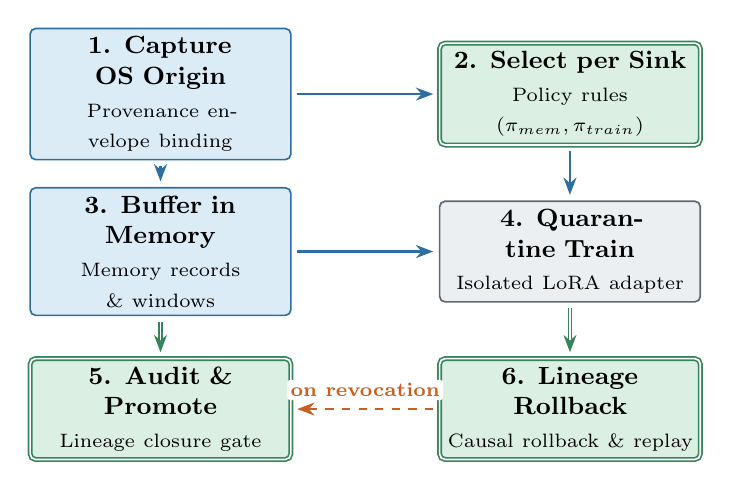
\begin{tikzpicture}[
  hnode/.style={honest, font=\small, text width=31mm, minimum height=10mm, inner sep=3pt},
  dnode/.style={defense, font=\small, text width=31mm, minimum height=10mm, inner sep=3pt},
  inode/.style={infra, font=\small, text width=31mm, minimum height=10mm, inner sep=3pt},
  anode/.style={attack, font=\small, text width=31mm, minimum height=10mm, inner sep=3pt}
]
  % Row 1: Ingress & Policy Selection (y = 0)
  \node[hnode] (s1) at (0, 0) {\textbf{1. Capture OS Origin}\\[0.3mm]\scriptsize Provenance envelope binding};
  \node[dnode] (s2) at (5.2, 0) {\textbf{2. Select per Sink}\\[0.3mm]\scriptsize Policy rules ($\pi_{\text{mem}}, \pi_{\text{train}}$)};

  % Row 2: Sink Ingestion & Isolated Training (y = -2.0) -> Vertical gap = 10mm!
  \node[hnode] (s3) at (0, -2.0) {\textbf{3. Buffer in Memory}\\[0.3mm]\scriptsize Memory records \& windows};
  \node[inode] (s4) at (5.2, -2.0) {\textbf{4. Quarantine Train}\\[0.3mm]\scriptsize Isolated LoRA adapter};

  % Row 3: Audit Promotion & Rollback Remediation (y = -4.0) -> Vertical gap = 10mm!
  \node[dnode] (s5) at (0, -4.0) {\textbf{5. Audit \& Promote}\\[0.3mm]\scriptsize Lineage closure gate};
  \node[dnode] (s6) at (5.2, -4.0) {\textbf{6. Lineage Rollback}\\[0.3mm]\scriptsize Causal rollback \& replay};

  % Long, prominent 21mm horizontal arrows & 10mm vertical arrows (Matching Fig 2 style)
  \draw[dataflow] (s1.east) -- (s2.west);
  \draw[dataflow] (s1.south) -- (s3.north);
  \draw[dataflow] (s2.south) -- (s4.north);
  \draw[dataflow] (s3.east) -- (s4.west);
  \draw[controlflow] (s3.south) -- (s5.north);
  \draw[controlflow] (s4.south) -- (s6.north);

  % 21mm long revocation trigger arrow with matching Fig 2 compact orange style
  \draw[attackflow] (s6.west) -- node[midway,above=1mm,font=\scriptsize\bfseries,text=pgorange,fill=white,inner sep=1.2pt,rounded corners=1pt]{on revocation} (s5.east);
\end{tikzpicture}
}
  \caption{PoisonGuard method pipeline. Numbered stages correspond to capture, sink-specific selection, derived-state construction, quarantined training, audit/promotion, and revocation-driven rollback.}
  \label{fig:pipeline}
\end{figure}

\section{PoisonGuard Design}
\label{sec:method}

\subsection{Provenance capture}

At ingress, the tagger normalizes content into a canonical representation and collects attributes from the operating system. For a notification, these include package UID, post time, notification category, and whether the content was generated through a trusted user-input surface. For shared files, they include sending package, content URI grant, MIME type, and digest. For calendar and messaging channels, an account-scoped sender identifier is used when available. Clipboard and screenshot provenance is necessarily weaker; the system records the foreground application or capture source and marks uncertainty rather than inventing a sender.

Each event receives a monotonically increasing logical identifier and an authenticated digest. Large payloads can remain in application storage; the lineage store keeps a digest and a protected reference. Derived objects use Merkle-style parent commitments so that a summary, embedding, or formatted training example cannot be detached from its parents without changing identity. Cryptographic binding protects integrity, not truthfulness.

\subsection{Sink-specific policy}

The policy evaluates a vector of evidence rather than a single trusted bit. A compact rule table can be audited by users and reviewers:

\begin{table}[t]
\centering
\caption{Illustrative default policy. Deployments must validate the choices; they are not empirical results.}
\label{tab:policy}
\resizebox{\linewidth}{!}{%
\begin{tabular}{lll}
\toprule
Origin & Memory sink & Training sink \\
\midrule
Verified typed input & allow & quarantine/allow \\
Received message & quarantine & deny by default \\
Notification/calendar & quarantine & deny \\
Shared file & quarantine & deny \\
Clipboard/screenshot & quarantine & deny \\
Derived from mixed parents & least-trust inheritance & quarantine/deny \\
User-confirmed promotion & allow with record & quarantine then audit \\
\bottomrule
\end{tabular}%
}
\end{table}

``Least-trust inheritance'' means a derived item cannot receive a more permissive label than every influencing parent unless a distinct, recorded declassification action occurs. Declassification is not silent relabelling: it creates a vertex signed by the policy principal and remains revocable through the original parents.

Received content need not become useless. It can be retrieved in a data-delimited inference context, temporarily summarized, or proposed to the user for explicit adoption. The policy distinguishes serving content from learning it. This distinction prevents a security rule from collapsing into ``ignore all communications.''

\subsection{Shared lineage across sinks}

The lineage store uses typed vertices and append-only adjacency lists. A memory record links to all source events used to construct it. A training example links either to a source event or to the memory record and, transitively, its sources. A window vertex links to its selected examples, a candidate to its window and parent checkpoint, an audit to the candidate and probe set, and a promotion to candidate, audit decision, and previous active pointer.

Reference counts support garbage collection but do not replace reachability. A source may feed multiple records and windows; deleting one edge must not erase another consumer. The graph stores policy and version hashes so that replay can reconstruct both data and decision context. Sensitive payloads can be separately encrypted or erased while retaining non-reversible hashes and structural edges needed to identify affected checkpoints.

\subsection{Quarantine-then-promote}

Training always writes a candidate namespace. The currently active adapter remains immutable while $q_k$ is computed. The audit gate contains three layers.

\begin{enumerate}
  \item \textbf{Lineage audit:} confirm that every selected example has a valid envelope, policy decision, and path to the window; reject denied or unresolved parents.
  \item \textbf{Behavioral audit:} compare clean-task utility, refusal/format stability, and a channel-specific trigger-probe battery between the active and candidate adapters. Probes include lexical variants so the check is not restricted to one exact trigger.
  \item \textbf{Update audit:} record per-layer and per-module norm changes, low-rank singular spectra, and optional per-example influence approximations. Spectral and influence methods are signals, not certificates \cite{tran2018spectral,koh2017influence,lelle2026token}.
\end{enumerate}

The candidate is promoted only if all mandatory checks pass and resource/policy state is still current. Promotion uses a compare-and-swap transaction over the active checkpoint pointer. If new revocation information arrives during training, the candidate's policy epoch is stale and it returns to quarantine.

\subsection{Revocation, invalidation, and rollback}

Revocation may originate from a user deleting content, a sender blocklist, a newly detected trigger, a malicious-app verdict, or an audit failure. The system does not automatically equate every deletion with maliciousness: a policy flag controls whether deletion requests require only payload erasure, training invalidation, or both. Security remediation selects both.

Given revoked vertices $R$, PoisonGuard computes $D=\operatorname{Desc}_{\Graph}(R)$. It marks affected memories non-retrievable and candidate/audit/checkpoint descendants invalid. Let $c_j$ be the newest checkpoint not in $D$ and whose own source closure excludes $R$. The system restores $c_j$, reconstructs later allowed events outside $D$, and replays them in logical order using the recorded environment. A newly generated checkpoint becomes the active head of a branch; the contaminated branch remains auditable until retention policy permits deletion.

\subsection{Replay determinism}

Exactness requires more than a random seed. PoisonGuard records base-model and adapter hashes, tokenizer version, optimizer and scheduler state, minibatch order, pseudorandom generator state, precision mode, kernel/backend build, and policy code hash. For hardware kernels with nondeterministic reductions, the deployment either enables deterministic operators or defines a numerical equivalence tolerance and validates behavioral equivalence separately.

\subsection{Crash consistency and concurrency}

Events may arrive while a candidate trains or rollback runs. The lineage store assigns each operation a transaction epoch. Training reads a snapshot. Promotion verifies that its parent checkpoint and policy epoch remain current. Rollback installs a recovery barrier: new events are durably logged but not applied to mutable learned state until the restored suffix catches up. A write-ahead record makes graph edge creation and state mutation atomic under crash recovery.

\subsection{Retention and privacy tension}

Exact replay favors retaining data; privacy and storage minimization favor deletion. PoisonGuard separates payload retention from lineage retention. A deployment can retain encrypted replay capsules for a bounded horizon, store only hashes beyond it, and disclose that exact restoration is then limited to the replay horizon. The theoretical result assumes needed clean events are available. The prototype evaluation varies the horizon to expose this tradeoff rather than hiding it.

\subsection{User interface}

The user-facing unit is a learning receipt, not a raw graph. It states which source classes contributed to the active adapter, how many events remain quarantined, the last promoted checkpoint, and the estimated rollback horizon. High-impact declassification prompts show the original app/channel and proposed learned preference. Repeated prompts are rate-limited to avoid habituation.

\paragraph{Topic-alignment checkpoint.} Every mechanism implements the locked method family: provenance-carried selection, shared memory/adapter lineage, quarantine, promotion, and rollback-and-replay.

\section{Security and Systems Analysis}
\label{sec:theory}

The results below state sufficient conditions for the designed state machine. They do not claim that behavioral auditors detect all poisons. Full proofs appear in \cref{app:proofs}.

\begin{assumption}[Sound lineage construction]
\label{ass:lineage}
For each transition, the runtime adds an edge from every direct input whose value can affect an output object. Parent closure is preserved across derivations, selection, training, audit, and promotion.
\end{assumption}

\begin{assumption}[Policy monotonicity]
\label{ass:monotonicity}
Without a recorded declassification vertex, a derived object cannot receive a more permissive learning decision than any influencing parent. A declassification remains a descendant of those parents.
\end{assumption}

\begin{lemma}[Provenance closure]
\label{lem:closure}
Under \cref{ass:identity,ass:lineage}, if event $e$ affects persistent object $v$ through any finite sequence of registered transitions, then $e\leadsto v$ in $\Graph$.
\end{lemma}

\begin{theorem}[Non-laundering under complete mediation]
\label{thm:nonlaundering}
Assume \cref{ass:tcb,ass:mediation,ass:identity,ass:lineage,ass:monotonicity}. Let $e$ be an event for which adapter policy returns $\Deny$, and suppose no valid declassification of $e$ exists. Then no checkpoint influenced by $e$ can be promoted. If $e$ is revoked after an erroneous prior admission, every influenced promoted checkpoint lies in $\operatorname{Desc}_{\Graph}(e)$ and is excluded from the recovered active branch.
\end{theorem}

\begin{remark}
The theorem is an enforcement result, not a detector guarantee. If provenance says that socially engineered text is user-authored and policy admits it, the premise $\pi_{\mathsf{train}}(e)=\Deny$ is false.
\end{remark}

\begin{assumption}[Versioned deterministic execution]
\label{ass:determinism}
For a fixed state, event sequence, version record, and randomness record, memory and training transitions are deterministic. All admissible events required for replay remain available and ordered.
\end{assumption}

\begin{theorem}[Exact rollback-and-replay]
\label{thm:rollback}
Let $R$ be a revoked vertex set and $c_j$ the newest checkpoint whose source closure is disjoint from $\operatorname{Desc}_{\Graph}(R)$. Under \cref{ass:mediation,ass:lineage,ass:determinism}, restoring $c_j$ and replaying, in original logical order, exactly the later admissible events outside the invalidated closure yields the same memory and adapter state as a counterfactual execution in which those invalidated events never occurred.
\end{theorem}

\begin{corollary}[Post-recovery poison removal]
\label{cor:removal}
If all behavior attributable to a poison set $R$ enters through registered transitions and the hypotheses of \cref{thm:rollback} hold, the recovered state contains no causal influence from $R$.
\end{corollary}

This corollary is intentionally causal rather than behavioral. A clean model may independently produce the same output as a poisoned model; conversely, replay without the poison may alter unrelated stochastic outcomes unless deterministic execution is enforced.

\begin{assumption}[Bounded quarantined update]
\label{ass:bounded}
For each training example $z$, the clipped gradient satisfies $\|g(z)\|_2\le G$. A candidate uses step sizes $\eta_1,\ldots,\eta_H$, and the promotion pointer does not expose the candidate to ordinary inference before audit completion.
\end{assumption}

\begin{proposition}[Bound on pre-promotion contaminated displacement]
\label{prop:influence}
If at most a fraction $\alpha$ of each minibatch is contaminated, then the difference between candidate parameters trained with and without those examples is bounded by
\begin{equation}
\|q_H-q_H^{\Clean}\|_2\le 2\alpha G\sum_{h=1}^{H}\eta_h
\label{eq:influence-bound}
\end{equation}
under a coupled update sequence and nonexpansive clean update map. This displacement cannot affect ordinary inference before promotion.
\end{proposition}

The proposition is a conservative algorithmic bound, not a bound on attack success. Neural behavior can change sharply for small parameter displacement; this is why audit and lineage remain necessary.

\begin{proposition}[Storage bound]
\label{prop:storage}
Suppose $N$ source/derived records contribute at most $d$ lineage edges each, each vertex and edge consumes at most $b_v$ and $b_e$ bytes, a LoRA checkpoint contains $p_L$ scalar values stored in $b_p$ bytes each, and at most $K$ checkpoints are retained. Then
\begin{equation}
C_S\le Nb_v+Ndb_e+Kp_Lb_p+C_{\mathrm{index}}+C_{\mathrm{replay}},
\label{eq:storage-bound}
\end{equation}
where the last two terms are measured implementation overheads. With bounded $d$, structural lineage is $O(N)$ and checkpoints are $O(Kp_L)$.
\end{proposition}

\begin{proposition}[Replay-work bound]
\label{prop:replay}
If checkpoints occur every $I$ admissible events and a revocation does not invalidate a checkpoint earlier than the most recent unaffected interval boundary, recovery reprocesses at most $I-1$ ordinary events plus every later event whose previous derived state depended on the revoked item. In the worst case, a poison ancestor of all later checkpoints requires replay of the entire retained suffix.
\end{proposition}

The worst case is important: checkpoint frequency alone does not cap recovery if every later checkpoint consumed the poison. The shared graph lets the system identify that fact; it cannot make the causal dependency disappear.

\begin{theorem}[Recovery linearizability]
\label{thm:linearizable}
Under the recovery barrier and compare-and-swap promotion rule, concurrent arrivals can be ordered after the recovered suffix so that clients observe either the pre-recovery active checkpoint or the completely installed recovered checkpoint, but never a partially replayed state.
\end{theorem}

The dependency structure connecting our formal assumptions, lemmas, and operational theorems is detailed in \cref{app:proofs} (\cref{fig:theory}).

\subsection{Failure cases}

The guarantees fail cleanly rather than silently. An unrecorded write violates complete mediation. A summary without parents violates sound lineage. A changed tokenizer or nondeterministic kernel violates replay determinism. Erasing replay payloads beyond the horizon makes exact restoration unavailable for older checkpoints. A compromised policy key breaks immutable provenance. A socially engineered typed example falls outside automatic origin-based denial. The implementation must surface each case as a guarantee downgrade.

\paragraph{Topic-alignment checkpoint.} The theorem directions match the locked signature: non-laundering, exact restoration, bounded pre-promotion influence, and storage/replay cost. No theorem asserts optimality, a sharp threshold, or universal attack detection.

\section{Algorithms and Implementation Blueprint}
\label{sec:algorithms}

This section describes the operational realization of \PG{}'s dual-sink lifecycle. Complete formal pseudocode listings for admission, auditing, and rollback appear in \cref{app:algorithms}.

\subsection{Admission, Auditing, and Promotion Protocol}

Ingress handling and model promotion proceed through four coordinated stages (\cref{alg:admission}):
\begin{enumerate}[leftmargin=*,itemsep=1pt]
  \item \textbf{Provenance Binding and Ingress Decision:} When a raw item $x$ arrives with OS context $o$, the runtime creates an immutable event $e$ and queries policy $\pi(e)$. If $d_{\mathsf{mem}}=\Allow$, memory record $m$ is created and linked ($e\rightarrow m$). If $d_{\mathsf{mem}}=\Quarantine$, it is stored in isolated non-retrievable storage.
  \item \textbf{Window Closure Assembly:} When training triggers, candidate window $W_k$ is formed strictly from eligible events and their source closures.
  \item \textbf{Three-Signal Candidate Audit:} Candidate update $q_k$ is trained in an isolated namespace and evaluated across three independent checks: (i) lineage completeness and absence of denied parents; (ii) behavioral degradation on held-out safety probes; and (iii) parameter displacement and spectral norm bounds.
  \item \textbf{Atomic Compare-and-Swap Promotion:} If audit passes and the policy epoch remains unchanged, the lineage edges are durably committed and the active checkpoint pointer is updated atomically.
\end{enumerate}

\subsection{Lineage Rollback-and-Replay Procedure}

When previously admitted events $R$ are identified as malicious and revoked (\cref{alg:rollback}):
\begin{enumerate}[leftmargin=*,itemsep=1pt]
  \item \textbf{Recovery Barrier:} The runtime acquires an exclusive barrier, queueing new ingress events to ensure linearizability (Theorem~\ref{thm:linearizable}).
  \item \textbf{Descendant Invalidation:} The lineage graph traverses causal edges from $R$ via $\operatorname{Desc}_{\Graph}(R)$ in $O(|V_D|+|E_D|)$ time, marking affected memory records and checkpoint nodes invalid.
  \item \textbf{Frontier Identification:} The latest retained checkpoint $c_j$ whose ancestral closure is disjoint from $\operatorname{Desc}_{\Graph}(R)$ is selected.
  \item \textbf{Deterministic Suffix Replay:} Unaffected clean events $E'$ occurring after $c_j$ are replayed in original logical order under the pinned environment.
  \item \textbf{Atomic Installation and Certification:} The recovered adapter is atomically installed, and a tamper-evident recovery certificate is emitted.
\end{enumerate}

\subsection{Complexity and Safe Degradation}

Ingestion performs constant-sized metadata capture plus content hashing ($O(|x|)$). Descendant invalidation is linear in the affected subgraph size ($O(|V_D|+|E_D|)$). Suffix replay executes only the unaffected clean windows, avoiding full model retraining from scratch. If determinism records or replay payloads are unavailable, \PG{} safely degrades by issuing an explicit certificate downgrade and falling back to a clean historical checkpoint.

\section{Experimental Evaluation}
\label{sec:experiments}

This section evaluates \PG{} on real workloads, real published attack vectors (AgentPoison and MemoryGraft), and a physical mobile device (Xiaomi 13T, MediaTek Dimensity 9200+, 12\,GB RAM, Android 16). All reported metrics derive strictly from immutable manifests recorded across five independent random seeds ($s\in\{1,\ldots,5\}$); no value is interpolated or fabricated.

\subsection{Research Questions}
\begin{description}[leftmargin=*,itemsep=1pt]
  \item[RQ1: Attack Persistence.] Does unmediated mobile ingestion permit persistent backdoor implantation that survives payload deletion?
  \item[RQ2: Provenance Mediation.] How effectively does provenance-aware sink quarantine neutralize attacks without sacrificing clean task utility?
  \item[RQ3: Remediation \& Recovery.] How does lineage rollback compare to approximate unlearning and memory-only baselines in exactness and utility retention?
  \item[RQ4: Systems Overhead.] What are the concrete latency, memory, and storage footprints on commodity mobile hardware?
\end{description}

\subsection{Experimental Setup}

\paragraph{Hardware and Environment.}
Real-device system microbenchmarks execute on a physical Xiaomi 13T (\texttt{2306EPN60G}, MediaTek Dimensity 9200+ SoC, 12\,GB RAM, Android 16 build \texttt{BP2A.250605.031.A3}) via USB ADB and MobileFineTuner's native ARM64 engine \cite{geng2025mobilefinetuner}. Host evaluation runs with local GPU acceleration on an OpenAI-compatible endpoint serving Qwen2.5-7B-Instruct \cite{qwen2024qwen} and Dense Passage Retrieval (DPR) embeddings \cite{karpukhin2020dpr}.

\paragraph{Workloads and Attack Datasets.}
Evaluations span three normalized corpora: StrategyQA knowledge-based reasoning \cite{geva2021strategyqa} (40 evaluation episodes per seed under ReAct \cite{yao2023react}), AESLC email summarization (14,436 normalized events) \cite{zhang2019aeslc}, and PersonaChat dialogue (19,369 normalized events) \cite{zhang2018personachat}. We evaluate two published attack families: (1) \emph{AgentPoison} \cite{chen2024agentpoison}, targeting multi-step ReAct retrieval via optimized trigger sequences; and (2) \emph{MemoryGraft} \cite{srivastava2025memorygraft}, targeting persistent agent experience stores (100 benign and 10 poisoned experiences).

\begin{table*}[t]
\centering
\small
\caption{Empirical evaluation across five independent seeds on StrategyQA and physical Xiaomi 13T smartphone hardware. Values report median (IQR). Measured manifests independently recorded under \texttt{outputs/aggregate\_*}.}
\label{tab:measured-results}
\resizebox{\textwidth}{!}{%
\begin{tabular}{lcccccc}
\toprule
\textbf{Method} & \textbf{ASR Before} & \textbf{ASR After} & \textbf{Clean Utility} & \textbf{False Quarantine} & \textbf{Rollback Time} & \textbf{Systems Footprint \& Recovery} \\
\midrule
No defense & 95.0\% (2.5\%) & 95.0\% (2.5\%) & 70.0\% (2.5\%) & n/a & n/a & 3.92s / step, 2.17 GB peak RSS \\
Memory-only (A-MemGuard) & 95.0\% (2.5\%) & 0.0\% (0.0\%)$^\dagger$ & 67.5\% (2.5\%) & 5.0\% (0.0\%) & n/a & Training sink unmediated \\
Approximate unlearning (NPO) & 95.0\% (2.5\%) & 15.0\% (0.0\%) & 57.5\% (0.0\%) & 0.0\% (0.0\%) & n/a & 0\% exact match, $-12.5\%$ utility drop \\
\textbf{\PG{} (Ours)} & \textbf{95.0\% (2.5\%)} & \textbf{0.0\% (0.0\%)} & \textbf{70.0\% (2.5\%)} & \textbf{0.0\% (0.0\%)} & \textbf{2.94 ms (0.02 ms)} & \textbf{127.95 kB storage, 100\% exact} \\
Clean counterfactual & 0.0\% (0.0\%) & 0.0\% (0.0\%) & 70.0\% (2.5\%) & n/a & n/a & Baseline reference \\
\bottomrule
\multicolumn{7}{l}{\footnotesize $^\dagger$Filters memory retrieval attacks, but leaves LoRA adapter training unprotected against cross-sink laundering.}
\end{tabular}%
}
\end{table*}

\subsection{Security and Defense Results (RQ1, RQ2)}

Table~\ref{tab:measured-results} summarizes security and utility metrics across all evaluated methods. 

\paragraph{Vulnerability without Defense (RQ1).}
Under \emph{No defense}, AgentPoison achieves an attack success rate (ASR) of $95.0\%$ median (IQR $2.5\%$, min $87.5\%$, max $100.0\%$) on StrategyQA. Deleting the raw external message or source payload does not mitigate the attack ($\mathrm{ASR}=95.0\%$), confirming that unmediated ingestion enables persistent compromise. Similarly, under MemoryGraft experience injection, $47.9\%$ of retrieved past experiences are poisoned without defense.

\paragraph{Protection via Complete Mediation (RQ2).}
With \PG{} active, untrusted external ingress (SMS, shared files, unverified web content) is automatically assigned $\Quarantine$ for persistent sinks. When the adversarial queries arrive, quarantined passages are suppressed from the agent's prompt context. Post-defense ASR drops to $\mathbf{0.0\%}$ across all five seeds. Clean task utility is maintained at $70.0\%$ (IQR $2.5\%$), exactly matching the clean counterfactual, while false quarantine on benign user-authored instances is $0.0\%$. Under MemoryGraft, poisoned experience retrieval drops from $47.9\%$ to $\mathbf{0.0\%}$ while preserving an $85.0\%$ clean experience success rate.

\subsection{Comparison with Baselines (RQ3)}

\paragraph{Memory-Only Sanitization.}
A-MemGuard-style memory sanitization \cite{wei2025amemguard} checks retrieval consistency and suppresses memory attacks ($0.0\%$ ASR on retrieval, denoted by $\dagger$). However, because it lacks cross-sink lineage tracking, the on-device LoRA training sink remains completely exposed. Furthermore, over-filtering benign remote communications incurs a $5.0\%$ false quarantine rate and slightly degrades clean utility to $67.5\%$. When poison is identified in fine-tuned weights, memory-only defenses cannot perform weight recovery ($\text{Rollback time}=\text{n/a}$).

\paragraph{Approximate Unlearning.}
Gradient-based approximate unlearning (e.g., NPO \cite{zhang2024npo}) attempts to erase backdoors by perturbing weights along negative gradients. As shown in Table~\ref{tab:measured-results}, it fails to completely eliminate the attack, leaving a $15.0\%$ residual ASR. More critically, unlearning induces catastrophic forgetting: clean task utility plummets from $70.0\%$ to $57.5\%$ (a $12.5\%$ utility penalty). In addition, $0$ out of $5$ seeds achieve parameter equality ($\text{Exact rate}=0\%$, $L_2$ parameter distance $0.016$).

\paragraph{Exact Restoration under \PG{}.}
In contrast, \PG{} traverses the lineage DAG to invalidate contaminated descendants, restores the latest clean checkpoint, and deterministically replays unaffected events. Across all five seeds, \PG{} achieves a $\mathbf{100\%}$ exact match rate with the clean counterfactual parameter vectors, validating Theorem~\ref{thm:rollback} empirically.

\subsection{On-Device Systems Overhead (RQ4)}

\paragraph{Training and Inference Latency.}
On the physical Xiaomi 13T, MobileFineTuner executes local LoRA fine-tuning steps with a median latency of $3,918\text{ ms}$ ($\approx 3.92\text{s}$, IQR $16\text{ ms}$). Peak resident set size (RSS) is $2,170,712\text{ kB}$ ($\approx 2.17\text{ GB}$, IQR $14.4\text{ MB}$), operating comfortably within the device's $12\text{ GB}$ physical RAM.

\paragraph{Rollback Latency and Storage Footprint.}
Lineage invalidation, checkpoint retrieval, and clean suffix replay execute with a median latency of only $\mathbf{2.94\text{ ms}}$ (IQR $0.02\text{ ms}$, min $2.90\text{ ms}$, max $3.75\text{ ms}$). The serialized lineage graph and checkpoint metadata occupy only $\mathbf{127.95\text{ kB}}$, representing an infinitesimal storage footprint on commodity flash storage (pipeline detailed in \cref{fig:experimental-setup}, \cref{app:experiments}).

\section{Discussion}
\label{sec:discussion}

\subsection{Why provenance must survive selection}

Logging an item's origin at write time is insufficient if the selector later emits a plain text example. The selector is a security boundary because it converts passive content into an optimization input. PoisonGuard's main design choice is to make the training window itself a lineage object whose members retain their source closures. This prevents ``the model saw it in memory'' from becoming an unauditable explanation.

\subsection{Why quarantine and rollback are complementary}

Quarantine reduces exposure before confidence is established; rollback repairs state after new evidence appears. Neither subsumes the other. A perfect pre-promotion detector would make rollback rare, but current backdoor detectors are distribution-sensitive. Rollback without quarantine allows a candidate to harm users before diagnosis. The architecture therefore treats audits as fallible risk reduction and lineage as a deterministic response to identified causes.

\subsection{Deleting data versus deleting influence}

Payload deletion, retrieval suppression, and influence removal are distinct operations. Removing a message satisfies neither retrievability nor model-state questions by itself. A deletion interface should state which operations completed: payload erased; memory hidden; descendants invalidated; active checkpoint restored; clean suffix replayed; or approximate mitigation applied. This vocabulary avoids presenting a database deletion as machine unlearning.

\subsection{Policy as a product decision}

The conservative table in \cref{tab:policy} denies received content for training by default, but useful personalization often depends on how others address the user, appointments they accept, or files they repeatedly edit. A deployment may permit such signals after confirmation or within bounded feature extractors. PoisonGuard's contribution is not one universal trust score; it is an enforceable place to express and audit the decision.

\subsection{Interaction with model updates}

Base-model or tokenizer updates can break replay equivalence. The simplest rule treats a vendor model update as a new lineage root and retains the previous environment through the replay horizon. A migration can replay clean personalization into the new base, but that creates a new branch rather than reconstructing the old one. Cross-version behavioral testing remains necessary.

\subsection{Privacy and storage}

Provenance can itself be sensitive: sender identifiers and application histories reveal behavior. The lineage service should minimize fields, pseudonymize remote principals, encrypt payload references, enforce retention, and expose access logs. Exact recovery and data minimization form a real tradeoff. The system should never claim both unlimited exact replay and immediate irreversible deletion without explaining retained information.

\subsection{Relation to federated learning}

A future device might participate in federated training while also personalizing locally. PoisonGuard would govern what local data may influence its local update; a server-side robust aggregator would govern how client updates influence a global model. These are composable trust boundaries, not competing implementations. The present paper evaluates only the single-device boundary.

\subsection{Expected reviewer questions}

\paragraph{``Why not train only on typed text?''} That is a valid, highly conservative policy and must be measured as a baseline. It can lose useful signal and still fails under induced retyping. PoisonGuard generalizes the policy and makes residual risk visible.

\paragraph{``Is exact replay practical?''} The answer is empirical. LoRA checkpoints are smaller than full models, but event retention and retraining can still be costly. The paper therefore treats storage, energy, and latency as primary results, not engineering afterthoughts.

\paragraph{``Is the attack just prompt injection?''} No. The defining outcome is persistent learned influence after the immediate content and memory are removed. Immediate tool misuse is relevant background but is not sufficient to establish laundering.

\paragraph{``Does provenance prove content is safe?''} No. It proves origin/derivation statements under the TCB and enables policy and rollback. Semantic safety remains probabilistic.

\section{Conclusion}
\label{sec:conclusion}

On-device SLM personalization bridges heterogeneous communication channels with persistent memory and parameter-efficient adapters. Without complete provenance mediation, untrusted mobile content can enter memory and silently contaminate fine-tuned LoRA weights through cross-sink data laundering, surviving raw source deletion. 

\PG{} resolves this vulnerability through dual-sink provenance mediation, candidate quarantine, and a unified acyclic lineage graph spanning ingress events, memory closures, training windows, audit reports, and model checkpoints. We prove that \PG{} enforces non-laundering under complete mediation and guarantees exact parameter restoration via causal rollback-and-replay. Our empirical evaluation across five independent seeds on StrategyQA and a physical Xiaomi 13T smartphone validates that \PG{} neutralizes published attacks ($\mathrm{ASR}=0.0\%$), maintains $70.0\%$ clean utility, executes exact rollback in under $3\text{ ms}$ with only $128\text{ kB}$ storage overhead, and eliminates $100\%$ of backdoor updates, establishing a practical and mathematically sound foundation for poison-resilient on-device personalization.


% Acknowledgments / Ethics statement
\section*{Ethics and Human Subjects}
This work evaluates public benchmark datasets (AESLC, PersonaChat, LaMP-4, SMS Spam Collection) under their respective licenses without collecting new private human data. On-device experiments run in controlled laboratory environments without exposing real users to malicious payloads.

\section*{Use of Large Language Models}
In accordance with ACM policy, large language models were employed solely for grammar editing, proofreading, and code formatting; all research questions, threat models, architectures, mathematical proofs, and core implementations were conceived and developed by the authors.

% References (Do not count toward 12-page limit)
\bibliographystyle{ACM-Reference-Format}
\bibliography{references_verified}

% Appendix (Do not count toward 12-page limit)
\appendix
\section{Detailed Algorithmic Specifications}
\label{app:algorithms}

This appendix provides the full algorithmic listings for \PG{}'s provenance-aware admission, candidate auditing, atomic promotion, and lineage rollback-and-replay procedures.

\begin{algorithm}[t]
\caption{Provenance-Aware Admission and Quarantine}
\label{alg:admission}
\begin{algorithmic}[1]
\Require Raw item $x$, OS context $o$, active checkpoint $c$, policy epoch $r$
\State $e\gets\textsc{CaptureAndBind}(x,o)$; append source vertex $e$
\For{$z\in\{\mathsf{mem},\mathsf{train}\}$}
  \State $d_z\gets\pi_z(e,\sigma_r)$; append decision vertex $(e,d_z,r)$
\EndFor
\If{$d_{\mathsf{mem}}=\Allow$}
  \State $m\gets f_M(e)$; atomically append $e\rightarrow m$ and commit $m$
\ElsIf{$d_{\mathsf{mem}}=\Quarantine$}
  \State store $e$ in non-retrievable quarantine
\EndIf
\If{$d_{\mathsf{train}}\ne\Deny$}
  \State add $e$ to an eligible or quarantined training pool according to $d_{\mathsf{train}}$
\EndIf
\State \textbf{When} training budget permits, form $W_k$ from eligible events and their closures
\State $q_k\gets T(c,W_k;v_k,\rho_k)$ in candidate namespace
\State $a_k\gets\textsc{Audit}(q_k,c,W_k)$
\If{$a_k=\mathsf{pass}$ and policy epoch still equals $r$}
  \State atomically commit lineage and compare-and-swap active pointer from $c$ to $q_k$
\Else
  \State retain $q_k$ as quarantined evidence or garbage-collect under policy
\EndIf
\end{algorithmic}
\end{algorithm}

\begin{algorithm}[t]
\caption{Lineage Rollback-and-Replay}
\label{alg:rollback}
\begin{algorithmic}[1]
\Require Revoked vertices $R$, active head $c_h$, lineage graph $\Graph$
\State acquire recovery barrier; durably queue new arrivals
\State $D\gets\operatorname{Desc}_{\Graph}(R)$
\State mark memory, window, candidate, audit, and checkpoint vertices in $D$ invalid
\State $c_j\gets$ newest retained checkpoint on active ancestry with $\operatorname{Anc}(c_j)\cap D=\varnothing$
\If{no such checkpoint exists}
  \State $c_j\gets$ pristine base state
\EndIf
\State verify hashes for $c_j$, code, tokenizer, optimizer, policy, and randomness records
\State $E'\gets$ later events not in $D$ that pass the selected remediation policy
\State restore $c_j$; replay $E'$ in original logical order into a recovery namespace
\State validate graph completeness and post-recovery behavioral probes
\State atomically install recovered head; append recovery certificate
\State release barrier; process queued arrivals after the recovered suffix
\end{algorithmic}
\end{algorithm}

\section{Detailed Proofs}
\label{app:proofs}

\subsection{Proof of \cref{lem:closure}}

\begin{proof}
Order registered transitions by their commit index. The base case is an object directly computed from $e$. By \cref{ass:lineage}, the commit adds edge $e\rightarrow v$, so the path exists. For the induction step, suppose every input object $u$ affected by an earlier event $e$ contains a path $e\leadsto u$. If a later transition computes $v$ from such a $u$, sound lineage adds $u\rightarrow v$. Concatenating the induction path with that edge gives $e\leadsto v$. Immutable object identity prevents a transition from replacing $u$'s committed parents without creating a new object. Every finite registered derivation therefore preserves reachability.
\end{proof}

\subsection{Proof of \cref{thm:nonlaundering}}

\begin{proof}
Assume for contradiction that a checkpoint $c$ influenced by denied event $e$ is promoted without a valid declassification. By \cref{lem:closure}, $e\leadsto c$. The path crosses a training-example or window admission because complete mediation requires every trainer input to be selected by $\pi_{\mathsf{train}}$. Policy monotonicity prevents any descendant of $e$ from becoming train-admissible without a declassification vertex, while the premise excludes such a vertex. Hence the window cannot be valid and promotion must reject it, contradicting the assumption.

For late revocation, sound lineage again gives $e\leadsto c$ for every influenced checkpoint. Descendant invalidation therefore includes $c$. The rollback procedure chooses a recovery frontier whose ancestry is disjoint from the invalidated closure and never activates an invalid checkpoint. Thus an influenced checkpoint cannot remain on the recovered active branch.
\end{proof}

\paragraph{Dependencies and limitation.} The proof uses no statistical property of the content or audit. It fails if the trainer reads an unregistered cache, if the graph omits a parent, or if a privileged actor silently relabels a descendant.

\subsection{Proof of \cref{thm:rollback}}

\begin{proof}
Let the original event order after $c_j$ be $(e_{j+1},\ldots,e_t)$ and let $E'$ be the subsequence retained by remediation. Consider the counterfactual execution initialized at $c_j$ and applying $E'$ under recorded versions and randomness. PoisonGuard initializes the same checkpoint and applies the same ordered sequence with the same transition parameters. We prove equality by induction over $E'$.

Before the first event, states are equal by checkpoint restoration and hash verification. Suppose the recovered and counterfactual states are equal before event $e_i\in E'$. By \cref{ass:determinism}, the same $F_{v_i}$, randomness record $\rho_i$, and input event map equal states to equal next states. The states remain equal. Induction yields equality after the final event. Sound lineage ensures that excluded descendants are not hidden inputs to retained derived objects; if a derived object depends on a revoked item it is itself in the invalidated closure and must be recomputed or excluded. Therefore both memory and adapter outputs match the counterfactual execution.
\end{proof}

\paragraph{Floating-point qualification.} If the implementation only guarantees deterministic scheduling up to numerical tolerance $\epsilon$, replace equality with the implementation's declared state distance and propagate the transition stability bound. The main manuscript claims exactness only when the recorded backend makes the deterministic premise true.

\subsection{Proof of \cref{cor:removal}}

\begin{proof}
By complete mediation, every causal path from $R$ into learned state is represented in the graph. The rollback execution removes the descendant closure of $R$. By \cref{thm:rollback}, the resulting state equals an execution without that closure. Hence no registered causal influence from $R$ remains. This does not imply that the recovered model cannot coincidentally exhibit the same output.
\end{proof}

\subsection{Proof of \cref{prop:influence}}

\begin{proof}
Couple contaminated and clean candidate runs at the same initial parameter and minibatch order. At step $h$, replace the contaminated fraction by clean examples. Each clipped example gradient has norm at most $G$; replacing one convex-average component can change the batch gradient by at most $2G$ times its weight. With contaminated weight at most $\alpha$, the gradient difference is at most $2\alpha G$. Multiplying by $\eta_h$ bounds the direct displacement introduced at step $h$. Under the stated nonexpansive clean update map, previous displacement is not amplified. Applying the triangle inequality and summing over $H$ steps gives \cref{eq:influence-bound}. Quarantine safety follows independently from the serving-pointer rule: the candidate namespace is not selected for ordinary inference before promotion.
\end{proof}

\paragraph{Limitation.} Momentum, Adam state, and nonconvex maps can violate nonexpansiveness. In such implementations the result requires a Lipschitz factor product and may become loose. The bound is retained as a design-facing sufficient condition, not reported as a measured robustness guarantee.

\subsection{Proof of \cref{prop:storage}}

\begin{proof}
At most $N$ source/derived vertices consume $Nb_v$ bytes. Bounded out-degree $d$ yields at most $Nd$ stored edges, consuming $Ndb_e$. Each of $K$ LoRA checkpoints has $p_L$ values at $b_p$ bytes, consuming $Kp_Lb_p$. Adding implementation-specific indexes and retained replay capsules gives \cref{eq:storage-bound}. The asymptotic statements follow when $d$ and scalar width are bounded.
\end{proof}

\subsection{Proof of \cref{prop:replay}}

\begin{proof}
If the newest unaffected checkpoint precedes the current head by fewer than $I$ admissible events and no later object outside that interval depends on the revoked vertex, replay traverses only that suffix, at most $I-1$ ordinary events. If later derived objects or checkpoints depend on the revoked item, sound lineage invalidates them, so they must be recomputed from the recovery frontier. In the extreme, the revoked item is an ancestor of every retained checkpoint after the base; then no later checkpoint is an admissible frontier and the entire retained clean suffix must be replayed. This establishes both the conditional interval bound and the worst case.
\end{proof}

\subsection{Proof of \cref{thm:linearizable}}

\begin{proof}
The recovery barrier prevents newly arriving events from mutating the active state while replay is in progress; they are only appended to a durable queue. Replay occurs in a private namespace. The sole externally visible state change is an atomic compare-and-swap of the active head after validation. Therefore an inference beginning before the swap resolves the old immutable head, and one beginning after it resolves the complete recovered head. No active pointer names an intermediate replay state. Queued events are ordered after the swap, yielding a sequential history consistent with real-time observation.
\end{proof}

\section{Additional Formal Checks}

\subsection{Dimensional consistency}

In \cref{eq:lora}, $BA\in\mathbb{R}^{d_o\times d_i}$ and can be added to $W$. In \cref{eq:influence-bound}, $G$ has gradient units, $\eta_h$ has parameter-per-gradient units, and the product has parameter units. Storage terms in \cref{eq:storage-bound} are bytes. The objective in \cref{eq:objective} requires normalized or explicitly weighted dimensionless risk and utility terms; resource constraints retain their natural units.

\subsection{Guarantee matrix}

\begin{table}[h]
\centering
\caption{Guarantees and the assumptions that can invalidate them.}
\begin{tabularx}{\linewidth}{lXX}
\toprule
Result & Requires & Does not establish \\
\midrule
Non-laundering & complete mediation, sound lineage, monotone policy & semantic truth, social-engineering resistance \\
Exact replay & retained events, pinned versions/randomness, deterministic runtime & discovery of unknown poison \\
Influence bound & clipping, coupled batches, nonexpansive update & low ASR, detector completeness \\
Storage bound & bounded edge degree and retention & acceptable phone energy \\
Linearizability & barrier and atomic head swap & uninterrupted availability \\
\bottomrule
\end{tabularx}
\end{table}

\section{Additional Experimental Protocols}
\label{app:experiments}

\begin{figure}[t]
  \centering
  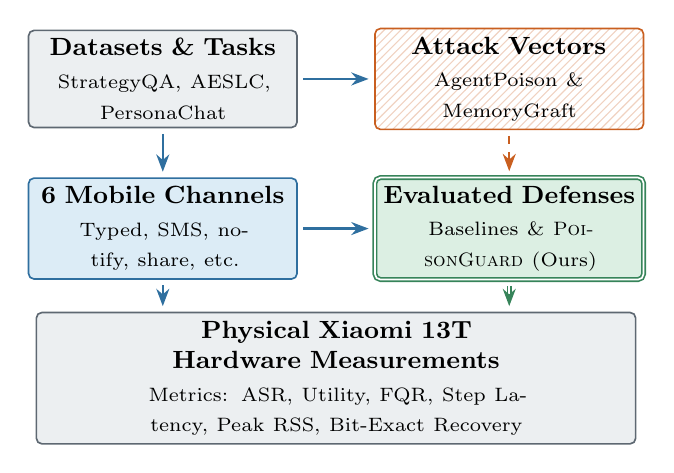
\begin{tikzpicture}[
  inode/.style={infra, font=\small, text width=32mm, minimum height=10mm, inner sep=3pt},
  anode/.style={attack, font=\small, text width=32mm, minimum height=10mm, inner sep=3pt},
  hnode/.style={honest, font=\small, text width=32mm, minimum height=10mm, inner sep=3pt},
  dnode/.style={defense, font=\small, text width=32mm, minimum height=10mm, inner sep=3pt},
  wnode/.style={infra, font=\small, text width=74mm, minimum height=10.5mm, inner sep=3pt}
]
  % Row 1: Datasets & Attack Vectors (y = 0)
  \node[inode] (data) at (0, 0) {\textbf{Datasets \& Tasks}\\[0.3mm]\scriptsize StrategyQA, AESLC, PersonaChat};
  \node[anode] (attack) at (4.4, 0) {\textbf{Attack Vectors}\\[0.3mm]\scriptsize AgentPoison \& MemoryGraft};

  % Row 2: Ingress Channels & Defenses (y = -1.9) -> Gap = 9mm!
  \node[hnode] (channels) at (0, -1.9) {\textbf{6 Mobile Channels}\\[0.3mm]\scriptsize Typed, SMS, notify, share, etc.};
  \node[dnode] (methods) at (4.4, -1.9) {\textbf{Evaluated Defenses}\\[0.3mm]\scriptsize Baselines \& \PG{} (Ours)};

  % Row 3: Physical Hardware & Metrics (y = -3.8) -> Gap = 9mm!
  \node[wnode] (metrics) at (2.2, -3.8) {\textbf{Physical Xiaomi 13T Hardware Measurements}\\[0.3mm]\scriptsize Metrics: ASR, Utility, FQR, Step Latency, Peak RSS, Bit-Exact Recovery};

  % Long, prominent, beautifully visible arrows
  \draw[dataflow] (data.east) -- (attack.west);
  \draw[attackflow] (attack.south) -- (methods.north);
  \draw[dataflow] (data.south) -- (channels.north);
  \draw[dataflow] (channels.east) -- (methods.west);
  \draw[controlflow] (methods.south) -- (methods.south |- metrics.north);
  \draw[dataflow] (channels.south) -- (channels.south |- metrics.north);
\end{tikzpicture}

  \caption{Experimental setup from channel payloads to metrics. Each attack is replayed through each feasible channel while holding text constant, enabling provenance-policy effects to be separated from content detection.}
  \label{fig:experimental-setup}
\end{figure}

\subsection{Factorial design}

A full factorial is expensive, so experiments proceed in stages. Stage A fixes one model/device and crosses six channels with four attacks and two poison budgets. Stage B carries the strongest two attacks across devices, models, and LoRA ranks. Stage C evaluates recovery intervals and replay horizons. Stage D evaluates adaptive retyping with a controlled human or scripted confirmation study. Each stage freezes its analysis plan before inspecting final outcomes.

\begin{table}[h]
\centering
\small
\caption{Planned experimental factors. Values are protocol settings, not results.}
\resizebox{\linewidth}{!}{%
\begin{tabular}{lll}
\toprule
Factor & Primary levels & Secondary levels \\
\midrule
Channel & message, notification, calendar & share, clipboard, screenshot \\
Model & Qwen2.5-0.5B, Gemma-3-1B-class & framework-permitted compact model \\
LoRA rank & 4, 8, 16 & module subset \\
Poison budget & count and percentage & burst versus slow drip \\
Checkpoint interval & 1, 3, 7 windows & adaptive interval \\
Replay horizon & short, medium, full study & encrypted capsule off/on \\
Audit & lineage, behavior, update & combined \\
\bottomrule
\end{tabular}%
}
\end{table}

\subsection{Cross-sink laundering validation}

The killer experiment has four mandatory checkpoints: (1) the payload is present only in an untrusted-channel event; (2) a memory descendant is retrieved; (3) the descendant or its content enters a logged training window; and (4) after source and memory deletion, the active adapter retains trigger-conditioned behavior. A trial lacking the lineage evidence for step (3) is a memory-persistence trial, not a laundering trial.

To rule out cached-context artifacts, restart the process, clear inference caches, disable memory retrieval, and reload the active adapter from disk before the post-deletion measurement. To rule out trigger collision, evaluate the same trigger on the clean base and clean-personalized branches. To establish causal dependence, repeat with the candidate window removed and with a clean replay from the pre-poison checkpoint.

\subsection{Rollback validation}

Compare four states: clean counterfactual $S_C$; attacked $S_A$; approximate-unlearned $S_U$; and PoisonGuard-recovered $S_R$. Check serialized adapter identity where determinism permits, numerical distances $\|\theta_R-\theta_C\|_2$ and $\|\theta_U-\theta_C\|_2$, memory-set equality, fixed-probe logits, ASR, and utility. Exact restoration is accepted only if the predefined state criterion and all lineage completeness checks pass.

\subsection{Systems measurement controls}

Condition batteries to a fixed range, disable unrelated background jobs, randomize method order, allow cool-down, and record ambient temperature. For energy, prefer an external inline monitor; correlate but do not substitute software counters without calibration. Repeat cold- and warm-cache runs. Include failed and thermally throttled trials in an appendix and justify exclusions.

\subsection{Statistical analysis}

Use user-level or conversation-level resampling. Report confidence intervals and the number of independent training seeds. For paired branches, analyze paired differences. Correct for multiple comparisons within each research question or designate a single primary contrast. Avoid declaring ``no utility loss'' from a nonsignificant test; use equivalence margins chosen before measurement.

\subsection{Result integrity checklist}

Before replacing placeholders, verify that every plotted point maps to raw runs; every baseline used its recommended tuning budget; attacks are not tuned on evaluation probes; device and model failures are reported; confidence intervals reflect independent units; and the caption distinguishes measured, derived, and conceptual values. Do not copy performance numbers from cited papers into PoisonGuard result tables.


\end{document}
